\documentclass[12pt,a4paper]{article}

\usepackage[a4paper,margin=1in]{geometry}
\usepackage{graphicx}
\usepackage{booktabs}
\usepackage{amsmath,amssymb}
\usepackage{float}
\usepackage{hyperref}
\usepackage{xcolor}
\usepackage{listings}
\usepackage{enumitem}
\usepackage{fancyhdr}
\usepackage{longtable}

\hypersetup{colorlinks=true,linkcolor=blue,urlcolor=blue}

\pagestyle{fancy}
\fancyhf{}
\lhead{ICS1512}
\rhead{Machine Learning Algorithms Laboratory}
\cfoot{\thepage}

\lstset{
language=Python,
basicstyle=\ttfamily\small,
numbers=left,
frame=single,
breaklines=true,
showstringspaces=false
}

\begin{document}

\begin{tabular}{|p{4cm}|p{11cm}|}
\hline
Experiment No. & 4 \\ \hline
Experiment Title & Binary Classification using Linear and Kernel-Based Models
\footnote{\textbf{GitHub Repository: }\url{https://github.com/username/repository}}\\ \hline
Student Name & \\ Amilineni Gopika \hline
Register Number & 3122247001003 \\ \hline
Faculty & Dr. Poreddy Ajay Kumar Reddy \\ \hline
Submission Date & 14-08-26\\ \hline
\end{tabular}

\section{Objective}
To classify emails as spam or ham using Logistic Regression and Support Vector Machine (SVM)
classifiers, and to analyze the effect of hyperparameter tuning on classification performance.

\section{Problem Statement}
Email spam filtering is a binary classification problem in which each email must be labelled as
either \textit{spam} (unwanted/unsolicited mail) or \textit{ham} (legitimate mail).
\textbf{Input:} 57 numeric features extracted from the content of an email --- frequencies of
specific words and characters, and statistics on runs of consecutive capital letters.
\textbf{Output:} a binary class label, $1$ for spam and $0$ for ham.
\textbf{Objective:} train and tune a Logistic Regression classifier and an SVM classifier (across
four kernels) on the Spambase dataset, compare their performance using standard classification
metrics, and study how hyperparameter choices affect generalization.

\section{Dataset Description}
\begin{longtable}{|p{6cm}|p{8cm}|}
\hline
Dataset Name & Spambase \\ \hline
Dataset Source & UCI Machine Learning Repository / Kaggle (\url{https://www.kaggle.com/datasets/somesh24/spambase}) \\ \hline
Number of Samples & 4601 \\ \hline
Number of Features & 57 numeric features (48 word-frequency, 6 character-frequency, 3 capital-run-length) \\ \hline
Number of Classes & 2 (0 = Ham, 1 = Spam) \\ \hline
Missing Values & 2091 missing cells spread across all 57 feature columns (24--56 missing values per column, $\approx$0.5--1.2\% per column); no missing values in the target; 0 duplicate rows \\ \hline
Train-Test Split & 80\% train (3680 samples) / 20\% test (921 samples), stratified on class \\ \hline
\end{longtable}

Class balance: 2788 ham (60.6\%) and 1813 spam (39.4\%) emails --- a moderate imbalance that is
handled with stratified splitting and stratified 5-fold cross-validation rather than resampling.

\section{Exploratory Data Analysis}

\begin{figure}[H]
\centering
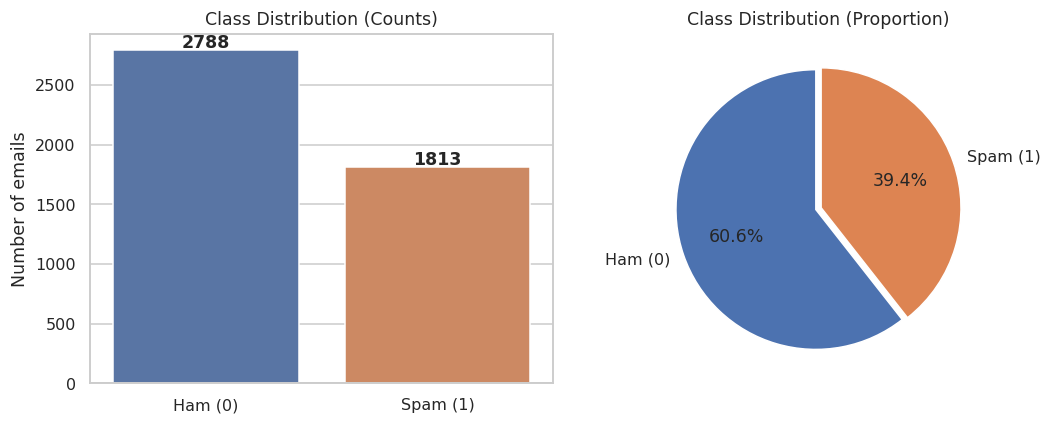
\includegraphics[width=0.85\linewidth]{images/class_distribution.png}
\caption{Class distribution of the Spambase dataset (counts and proportions).}
\end{figure}

\textbf{Inference:} The dataset is moderately imbalanced, with 60.6\% ham (2788 emails) and
39.4\% spam (1813 emails). This imbalance is not severe enough to require resampling techniques
such as SMOTE, but it does mean that accuracy alone can be slightly optimistic as a metric, so
precision, recall, F1-score and ROC-AUC are also reported throughout. Stratified splitting is
used for both the train-test split and all cross-validation folds to preserve this class ratio
consistently.

\begin{figure}[H]
\centering
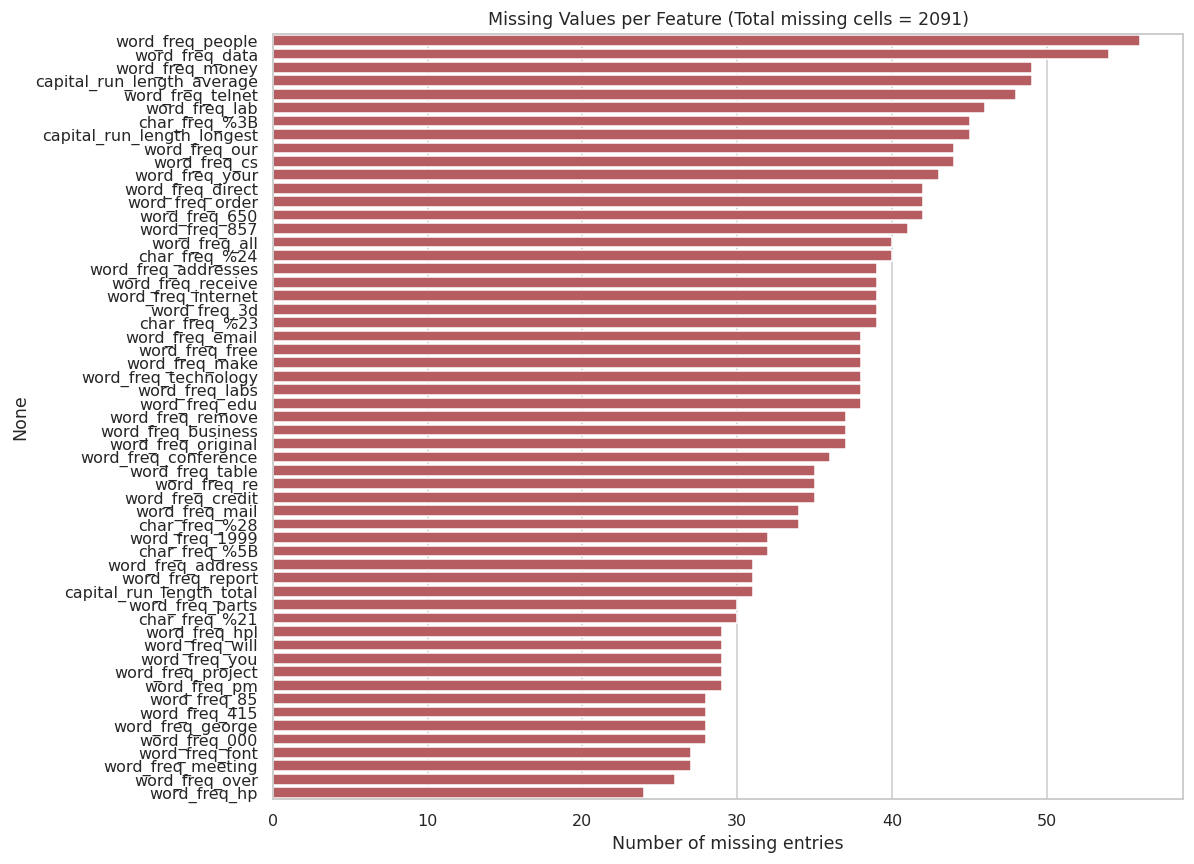
\includegraphics[width=0.95\linewidth]{images/missing_values.png}
\caption{Number of missing values per feature.}
\end{figure}

\textbf{Inference:} Every word/character-frequency feature carries a small number of missing
values (roughly 24 to 56 out of 4601 rows, i.e. 0.5\%--1.2\%), spread fairly evenly across
features rather than concentrated in a few columns or rows. No column is missing more than
$\approx$56 values, so the data can be safely repaired with simple median imputation without
materially distorting feature distributions. Because missingness is incidental and spread evenly,
there is no evidence of a systematic data-collection bias linked to class label.

\begin{figure}[H]
\centering
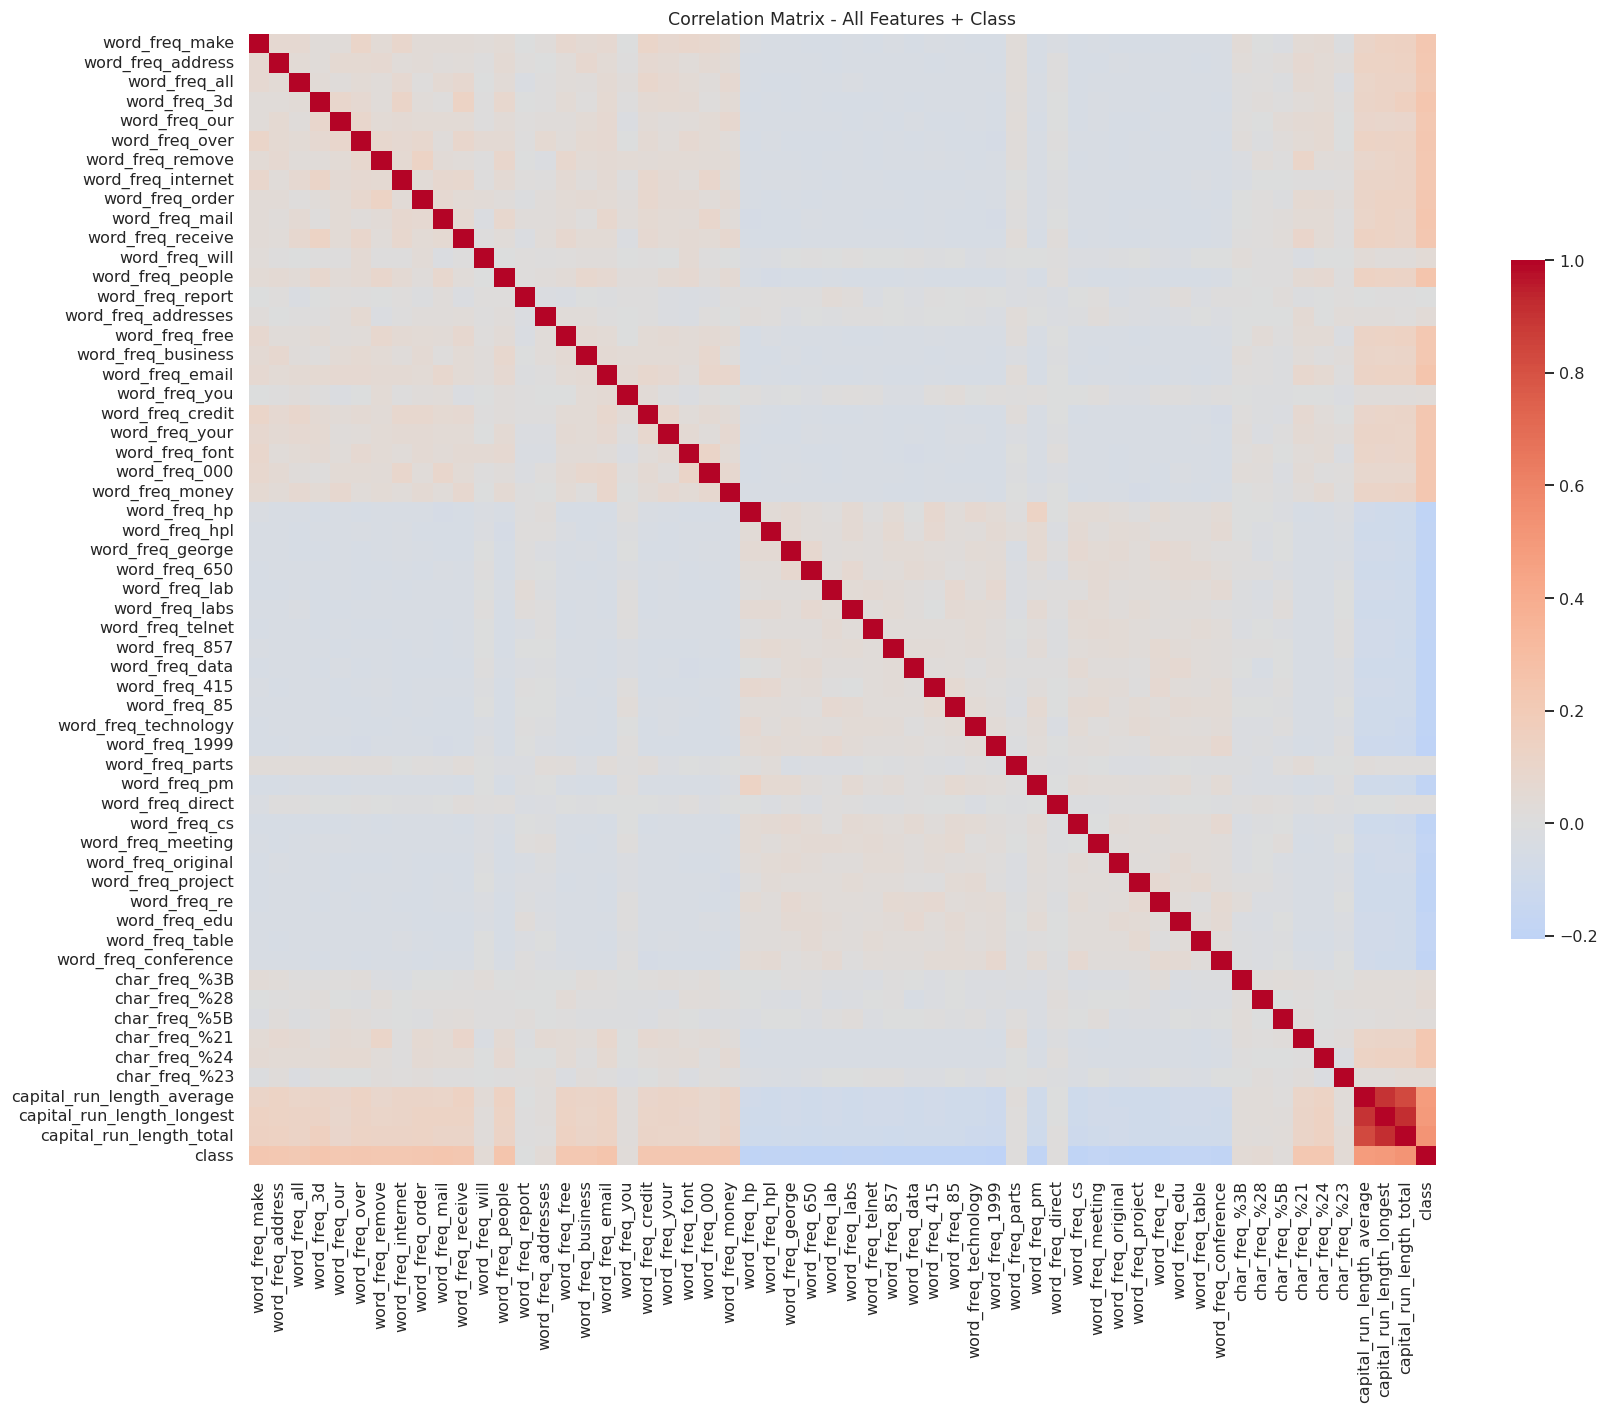
\includegraphics[width=\linewidth]{images/correlation_matrix.png}
\caption{Correlation matrix of all 57 features plus the class label.}
\end{figure}

\begin{figure}[H]
\centering
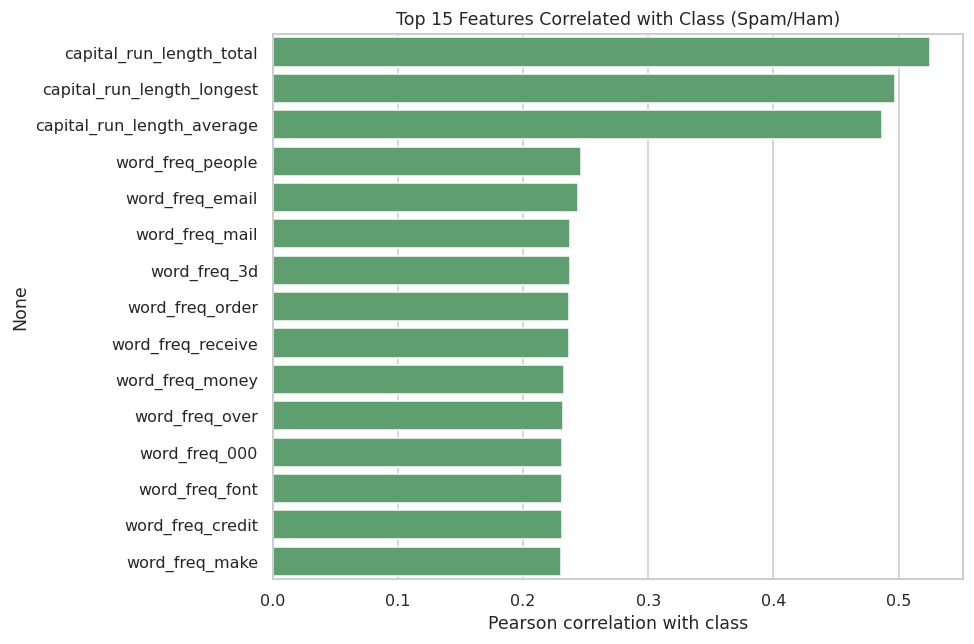
\includegraphics[width=0.85\linewidth]{images/top_correlated_features.png}
\caption{Top 15 features by absolute Pearson correlation with the class label.}
\end{figure}

\textbf{Inference:} Most individual word/character frequencies correlate only weakly with the
class label ($|r| < 0.3$), indicating that no single feature is a perfect spam signal --- the
classes are separated by the combination of many weak signals rather than one dominant feature.
The capital-letter run-length features (\texttt{capital\_run\_length\_total},
\texttt{\_longest}, \texttt{\_average}) show the strongest positive correlation with spam,
consistent with spam's heavy use of capitalized, emphatic text. Words such as
\texttt{word\_freq\_george}, \texttt{word\_freq\_hp} and \texttt{word\_freq\_hpl} (personal or
company-specific terms belonging to the original mailbox owner) correlate negatively with spam,
since their presence marks legitimate mail.

\begin{figure}[H]
\centering
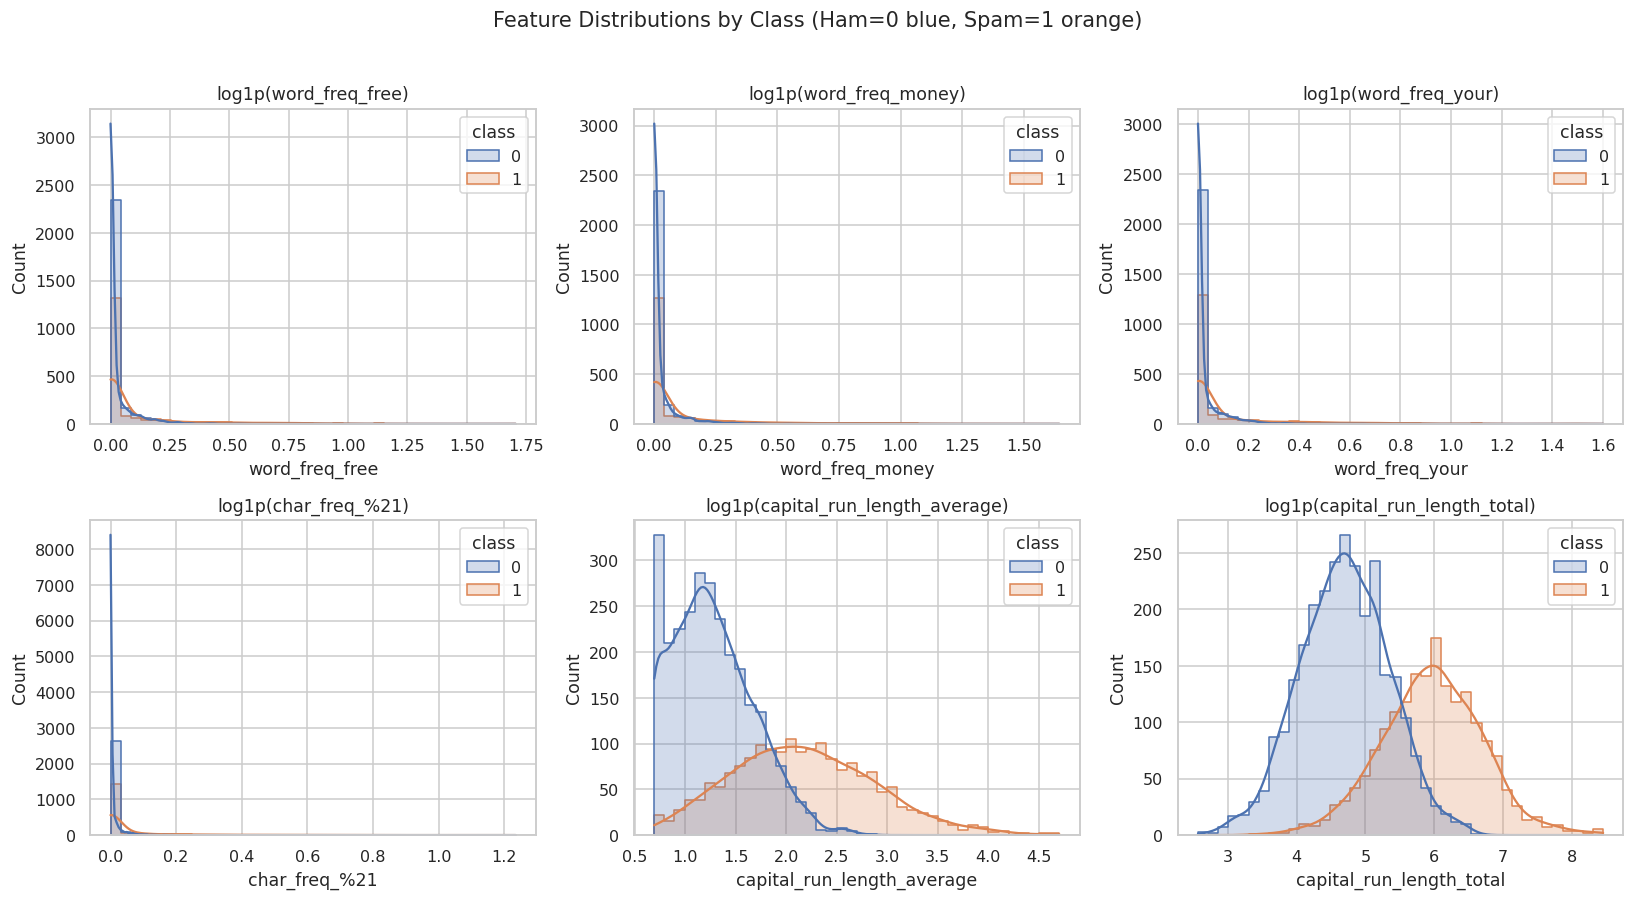
\includegraphics[width=\linewidth]{images/feature_distributions.png}
\caption{Distribution of selected features by class (log1p-transformed for visualization).}
\end{figure}

\textbf{Inference:} A log1p transform is applied purely for visualization since these frequency
features are heavily right-skewed with a large mass at zero. Spam emails are visibly shifted
right relative to ham for \texttt{word\_freq\_free}, \texttt{word\_freq\_money},
\texttt{word\_freq\_your} and \texttt{char\_freq\_\%21} (the ``!'' character) --- words and
punctuation typical of promotional or urgent language. The capital-run-length features show the
clearest visual separation between classes, reinforcing the correlation analysis above and
suggesting these will be influential predictors.

\section{Data Preprocessing}
\begin{itemize}
\item \textbf{Missing value handling:} all 2091 missing cells were imputed with the
\textbf{median} of their respective column, chosen for robustness against the strong right-skew
and outliers typical of frequency-based features.
\item \textbf{Encoding:} not required --- all 57 features are already numeric and the target is
already a binary 0/1 label.
\item \textbf{Feature scaling:} all features were standardized (zero mean, unit variance) using
\texttt{StandardScaler}, fitted on the training set only and applied to the test set, since both
Logistic Regression's regularization penalty and SVM's margin/kernel computations are
scale-sensitive.
\item \textbf{Train-test split:} 80\%/20\% split, stratified on the class label to preserve the
60.6\%/39.4\% ham/spam ratio in both subsets (train: 2230 ham / 1450 spam; test: 558 ham / 363
spam).
\item \textbf{Feature engineering:} not applied; the 57 pre-extracted features from the dataset
were used directly.
\end{itemize}

\section{Machine Learning Algorithms}

\subsection*{Logistic Regression}
\textbf{Working principle:} Logistic Regression models the probability that a sample belongs to
the positive class using a linear combination of features passed through the sigmoid function,
and applies a 0.5 probability threshold to obtain the predicted class.

\textbf{Mathematical formulation:}
\[
P(y=1\mid x) = \frac{1}{1+e^{-(w^Tx+b)}}
\]
The model is fit by minimizing the log-loss (binary cross-entropy), optionally with an L1 (Lasso)
or L2 (Ridge) penalty on the weights $w$ to control overfitting.

\textbf{Advantages:} fast to train, highly interpretable coefficients, outputs well-calibrated
probabilities, performs well when classes are close to linearly separable, and L1 regularization
gives automatic feature selection.

\textbf{Limitations:} assumes a linear decision boundary in feature space (or transformed
feature space), can underperform on strongly non-linear class boundaries, and is sensitive to
unscaled features and multicollinearity.

\subsection*{Support Vector Machine (SVM)}
\textbf{Working principle:} SVM finds the hyperplane that maximizes the margin between the two
classes; only the closest points (support vectors) determine the boundary. Kernels implicitly
map inputs into higher-dimensional spaces to allow non-linear separation.

\textbf{Mathematical formulation:} SVM solves
\[
\min_{w,b} \; \tfrac{1}{2}\lVert w \rVert^2 + C\sum_i \xi_i \quad \text{s.t. } y_i(w^T\phi(x_i)+b)\ge 1-\xi_i,\; \xi_i \ge 0
\]
where $\phi(\cdot)$ is the (implicit) kernel feature map, $C$ trades off margin width against
misclassification, and for RBF/polynomial/sigmoid kernels $\gamma$ controls the influence of
individual training points.

\textbf{Advantages:} effective in high-dimensional spaces, kernel trick allows flexible
non-linear boundaries, and the margin-maximizing objective often generalizes well.

\textbf{Limitations:} slower to train than Logistic Regression (especially with non-linear
kernels), less interpretable, more hyperparameters to tune ($C$, $\gamma$, kernel, degree), and
sensitive to feature scaling.

\section{Experimental Setup}
\begin{tabular}{ll}
\toprule
Python Version & 3.12.3 \\
Scikit-Learn Version & 1.8.0 \\
IDE & Jupyter Notebook \\
Operating System & Linux (Ubuntu 24.04) \\
Hardware & CPU-only execution \\
\bottomrule
\end{tabular}

\section{Hyperparameter Selection}

\textbf{Logistic Regression search space:}
\begin{tabular}{ll}
\toprule
Parameter & Value \\
\midrule
Regularization (penalty) & L1, L2 \\
C & 0.01, 0.1, 1, 10, 100 \\
Solver & liblinear, saga \\
\bottomrule
\end{tabular}

\vspace{0.4cm}
\textbf{SVM search space:}
\begin{tabular}{ll}
\toprule
Parameter & Value \\
\midrule
Kernel & Linear, Polynomial, RBF, Sigmoid \\
C & 0.1, 1, 10, 100 \\
$\gamma$ & scale, auto \\
Degree (Polynomial only) & 2, 3, 4 \\
\bottomrule
\end{tabular}

\vspace{0.4cm}
Both searches used exhaustive \textbf{Grid Search} with 5-fold stratified cross-validation,
optimizing for accuracy.

\section{Hyperparameter Tuning Results}

\begin{tabular}{llp{5.5cm}l}
\toprule
Model & Search Method & Best Parameters & Best CV Accuracy \\
\midrule
Logistic Regression & Grid Search & C=1, penalty=L1, solver=saga & 0.9861 \\
SVM & Grid Search & C=0.1, kernel=linear & 0.9859 \\
\bottomrule
\end{tabular}

\begin{figure}[H]
\centering
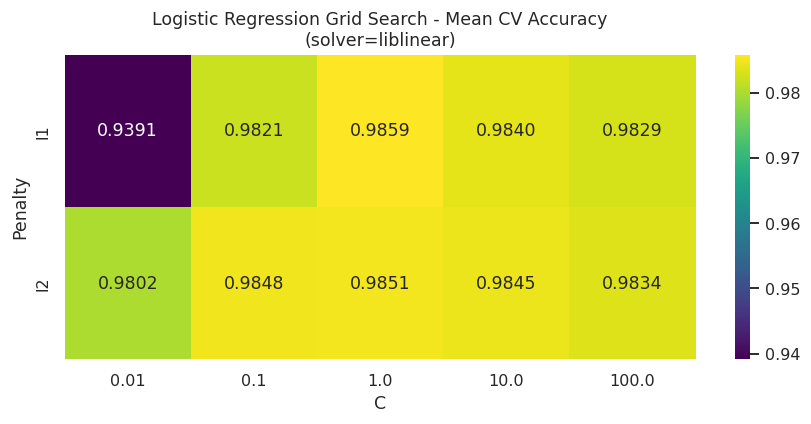
\includegraphics[width=0.8\linewidth]{images/lr_gridsearch_heatmap.png}
\caption{Logistic Regression grid search: mean 5-fold CV accuracy across C and penalty (solver=liblinear slice shown).}
\end{figure}

\textbf{Inference:} Accuracy is fairly flat across most $C$ values once $C \geq 0.1$, showing the
model is not highly sensitive to regularization strength beyond a minimum threshold, which
indicates the classes are close to linearly separable in the standardized feature space. Very
small $C$ (0.01, strong regularization) noticeably underperforms because it over-shrinks
coefficients and underfits. L1 and L2 perform almost identically at their respective optima, but
L1 was selected as it additionally yields a sparser, more interpretable model.

\begin{figure}[H]
\centering
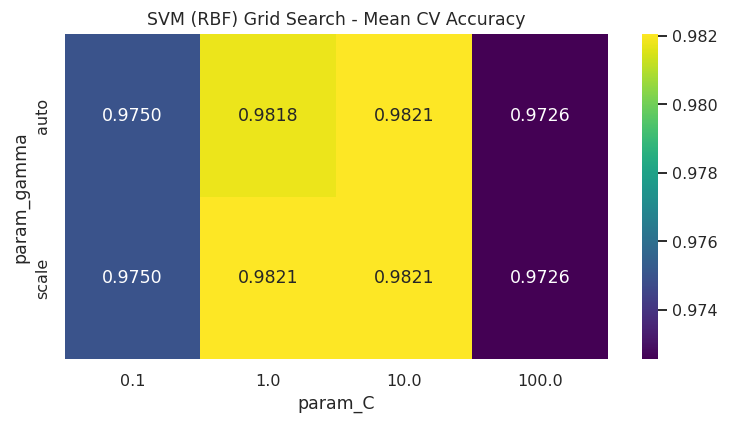
\includegraphics[width=0.7\linewidth]{images/svm_rbf_gridsearch_heatmap.png}
\caption{SVM (RBF kernel) grid search: mean 5-fold CV accuracy across C and $\gamma$.}
\end{figure}

\textbf{Inference:} For the RBF kernel, accuracy improves as $C$ increases from 0.1 up to about
10 (less regularization lets the margin fit the data more tightly), but plateaus or dips
slightly at $C=100$ --- an early sign of overfitting. \texttt{gamma=`scale'} is consistently at
least as good as \texttt{gamma=`auto'}. Across the full grid (all four kernels), the tuned
Linear kernel with a small $C$ narrowly won overall, reaffirming that this dataset is close to
linearly separable.

\section{Logistic Regression Performance}

\begin{tabular}{lcc}
\toprule
Metric & Baseline (default C=1, L2) & Tuned (Grid Search) \\
\midrule
Accuracy & 0.9794 & 0.9815 \\
Precision & 0.9804 & 0.9806 \\
Recall & 0.9669 & 0.9725 \\
F1 Score & 0.9736 & 0.9765 \\
ROC-AUC & --- & 0.9986 \\
Training Time (s) & 0.014 & 82.57 (full grid search) \\
\bottomrule
\end{tabular}

\section{SVM Kernel-wise Performance}

\begin{tabular}{lcccc}
\toprule
Kernel & Accuracy & F1 Score & Precision & Training Time (s) \\
\midrule
Linear & 0.9794 & 0.9737 & 0.9778 & 0.43 \\
Polynomial & 0.8730 & 0.8098 & 0.9881 & 1.89 \\
RBF & 0.9750 & 0.9679 & 0.9802 & 1.20 \\
Sigmoid & 0.9685 & 0.9594 & 0.9744 & 0.79 \\
\bottomrule
\end{tabular}

\begin{figure}[H]
\centering
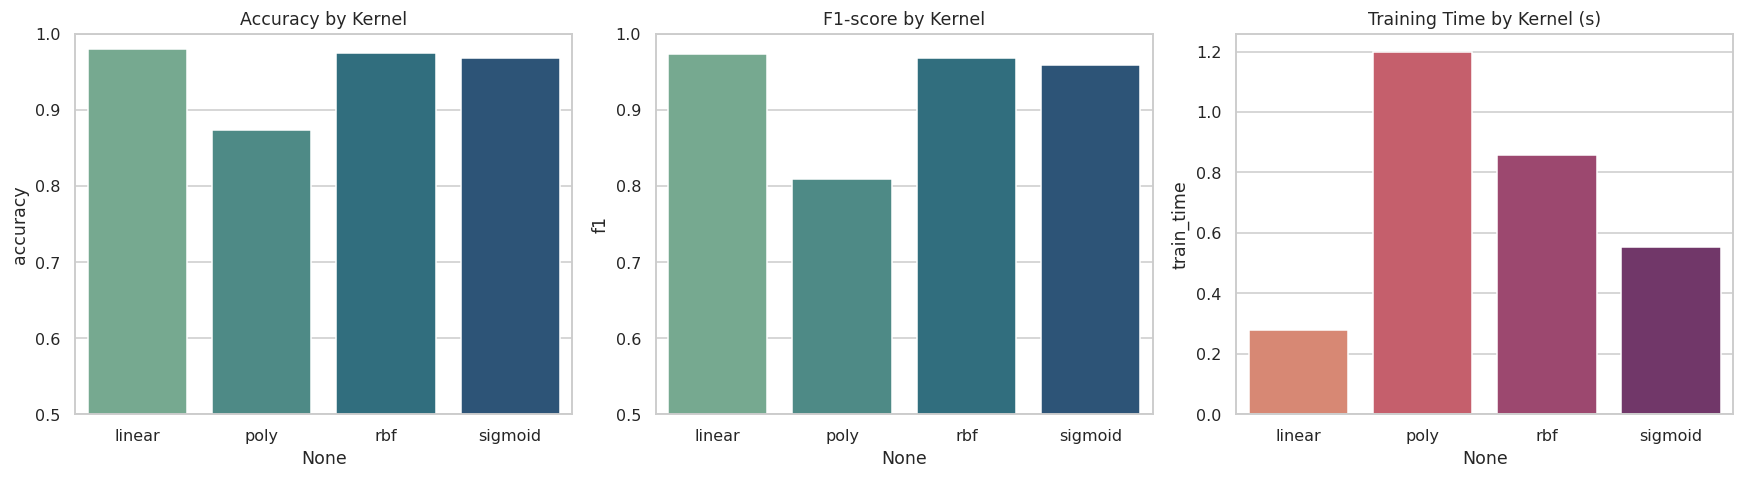
\includegraphics[width=\linewidth]{images/svm_kernel_comparison.png}
\caption{Baseline SVM performance and training time across the four kernels (default hyperparameters).}
\end{figure}

\textbf{Inference:} The Linear and RBF kernels perform best out-of-the-box ($\approx$97.5--97.9\%
accuracy), confirming that the classes are close to linearly separable, with RBF adding only a
marginal, non-significant benefit. The Polynomial kernel (default degree=3) performs
substantially worse ($\approx$87\% accuracy) with very high precision but low recall --- it is
missing many spam emails, likely due to its default hyperparameters, which motivated the tuning
step. The Sigmoid kernel sits in between the two extremes but trains fastest of the non-linear
kernels.

\textbf{Tuned SVM (best overall configuration, Linear kernel, C=0.1):}

\begin{tabular}{lc}
\toprule
Metric & Value \\
\midrule
Accuracy & 0.9761 \\
Precision & 0.9749 \\
Recall & 0.9642 \\
F1 Score & 0.9695 \\
ROC-AUC & 0.9982 \\
Training Time (full grid search, s) & 229.38 \\
\bottomrule
\end{tabular}

\section{K-Fold Cross-Validation Results (K = 5)}

\begin{tabular}{lcc}
\toprule
Fold & Logistic Regression & SVM \\
\midrule
Fold 1 & 0.9891 & 0.9864 \\
Fold 2 & 0.9837 & 0.9837 \\
Fold 3 & 0.9851 & 0.9837 \\
Fold 4 & 0.9891 & 0.9891 \\
Fold 5 & 0.9837 & 0.9864 \\
\midrule
Average & 0.9861 & 0.9859 \\
\bottomrule
\end{tabular}

\begin{figure}[H]
\centering
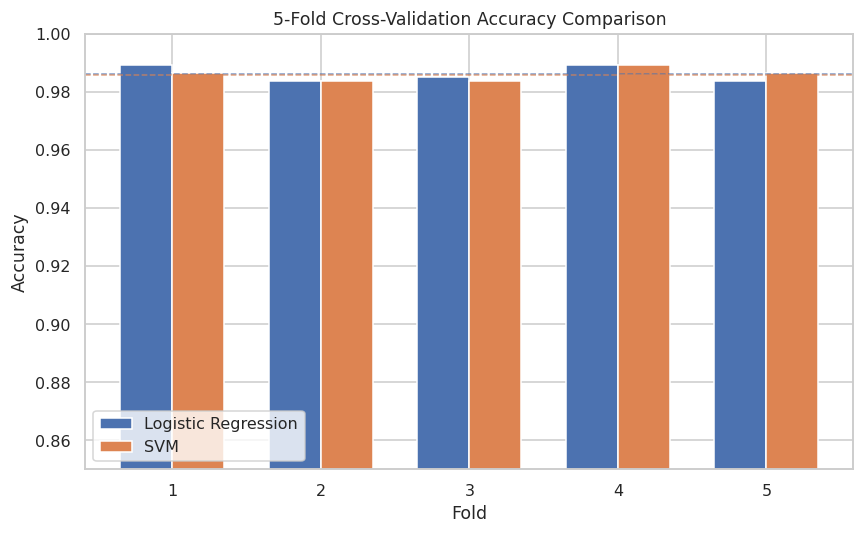
\includegraphics[width=0.85\linewidth]{images/cv_fold_comparison.png}
\caption{5-fold stratified cross-validation accuracy per fold for the tuned models.}
\end{figure}

\textbf{Inference:} Both models are extremely stable across folds --- accuracy varies by less
than 0.6 percentage points fold-to-fold for either model (LR std $\approx$0.0025, SVM std
$\approx$0.0020) --- so the single train/test split result generalizes reliably rather than
being an artifact of a favorable split. Logistic Regression's mean CV accuracy ($\approx$98.6\%)
is essentially tied with SVM's ($\approx$98.6\%), matching the held-out test-set comparison. The
low variance also suggests neither model is overfitting to particular folds of the training
data.

\section{Comparative Analysis}

\begin{tabular}{lcc}
\toprule
Criterion & Logistic Regression & SVM \\
\midrule
Test Accuracy & \textbf{0.9815} & 0.9761 \\
Model Complexity & Low & Higher (kernel-dependent) \\
Training Time & Low (0.01s baseline) & High (kernel/tuning dependent) \\
Interpretability & High & Lower \\
\bottomrule
\end{tabular}

\section{Result Visualization}

\begin{figure}[H]
\centering
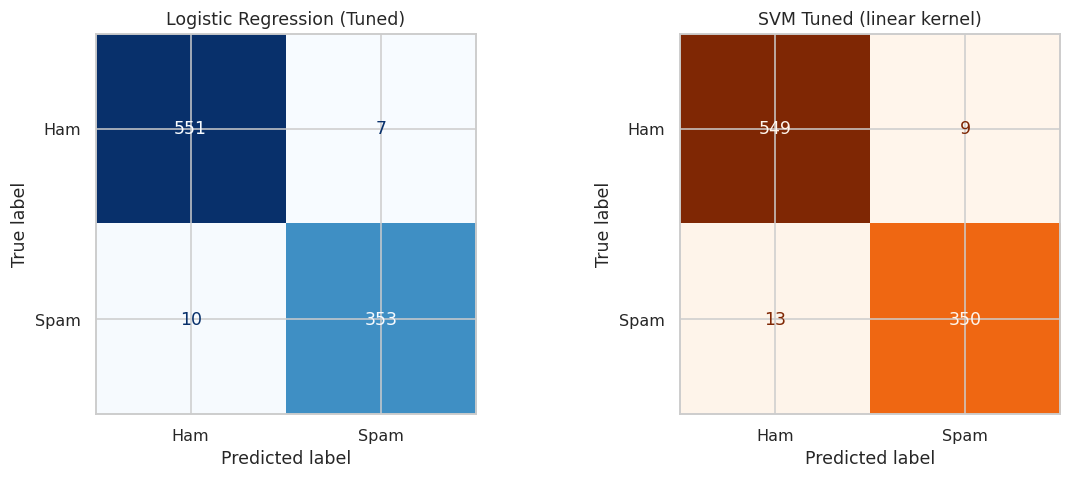
\includegraphics[width=\linewidth]{images/confusion_matrices.png}
\caption{Confusion matrices for the tuned Logistic Regression and tuned SVM (linear kernel) on the test set.}
\end{figure}

\textbf{Inference:} Both models produce very few false negatives (spam missed) and false
positives (ham misclassified as spam), which matters because false positives (losing a
legitimate email) are usually the costlier error in a real spam filter. Logistic Regression has
a slightly better false-negative count than the tuned SVM on this split, consistent with its
marginally higher recall (0.9725 vs 0.9642). Both confusion matrices are strongly
diagonal-dominant, reflecting the $>$97\% test accuracy achieved by both models.

\begin{figure}[H]
\centering
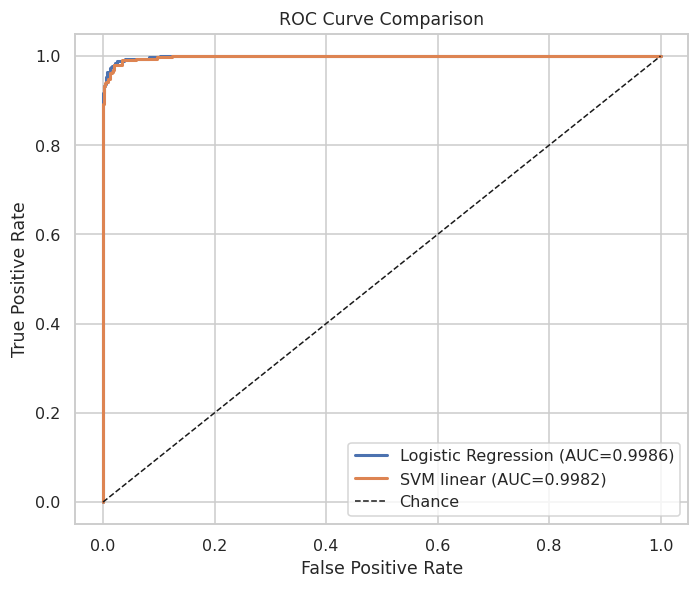
\includegraphics[width=0.7\linewidth]{images/roc_curve.png}
\caption{ROC curves for the tuned Logistic Regression and tuned SVM on the test set.}
\end{figure}

\textbf{Inference:} Both ROC curves hug the top-left corner almost perfectly, with AUC scores
above 0.998 for both classifiers (LR: 0.9986, SVM: 0.9982), indicating near-ideal class
separability at essentially every decision threshold. The curves are nearly indistinguishable,
confirming Logistic Regression and the tuned SVM are statistically comparable in ranking
performance on this dataset even though their decision boundaries are computed very differently.

\begin{figure}[H]
\centering
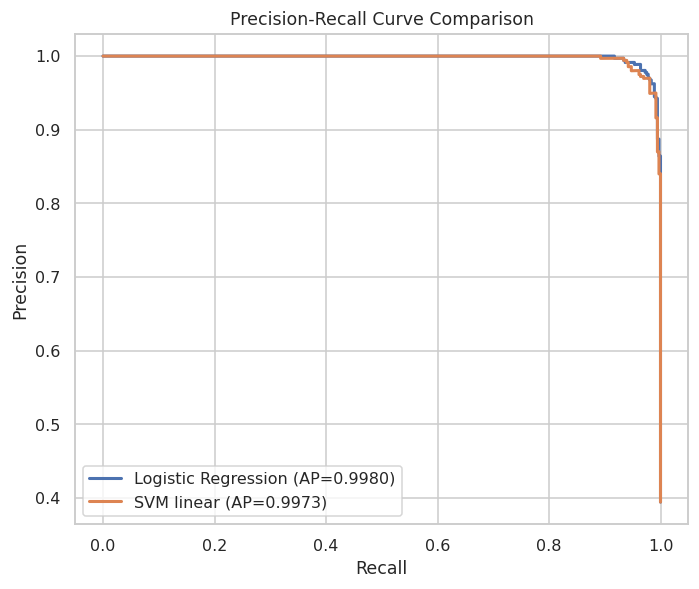
\includegraphics[width=0.7\linewidth]{images/pr_curve.png}
\caption{Precision-Recall curves for the tuned Logistic Regression and tuned SVM on the test set.}
\end{figure}

\textbf{Inference:} Average precision exceeds 0.997 for both models (LR: 0.9980, SVM: 0.9973),
meaning precision stays high across almost the entire recall range. This is important given the
moderate class imbalance (39\% spam): a model that only appeared to do well because of the
majority class would show a noticeably lower PR curve, which is not the case here. The
near-overlapping curves again show Logistic Regression and SVM trading blows rather than one
model dominating the other.

\begin{figure}[H]
\centering
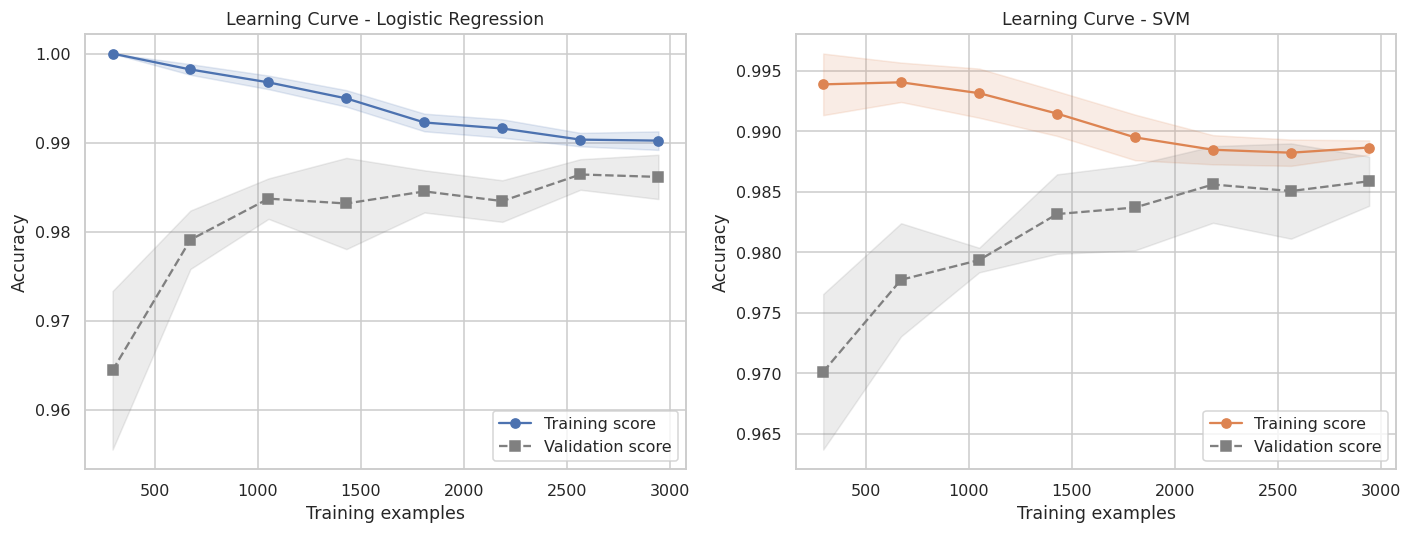
\includegraphics[width=\linewidth]{images/learning_curves.png}
\caption{Learning curves (training vs. 5-fold cross-validation accuracy) for both models.}
\end{figure}

\textbf{Inference:} Both learning curves converge quickly, with training and validation scores
nearly meeting after only $\approx$1500--2000 examples, indicating low variance (not
overfitting) and that the $\approx$3680-example training set is more than sufficient for both
models. The small, persistent gap between training and validation accuracy shows a minor amount
of bias/variance trade-off remains but is not concerning. Neither curve shows the validation
score still climbing at the full training size, so collecting more data would likely yield only
marginal further gains.

\begin{figure}[H]
\centering
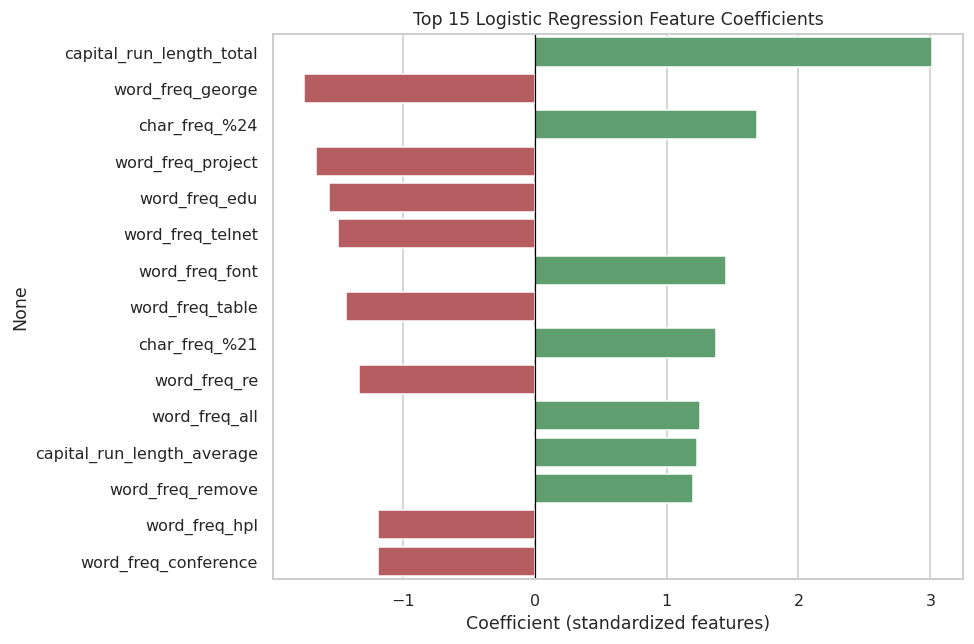
\includegraphics[width=0.85\linewidth]{images/feature_importance_lr.png}
\caption{Top 15 Logistic Regression coefficients (standardized features).}
\end{figure}

\textbf{Inference:} \texttt{capital\_run\_length\_total} has by far the largest positive
coefficient, confirming it as the single strongest driver of a spam prediction, consistent with
the EDA correlation analysis. Character/word features associated with promotional or urgent
language (\texttt{char\_freq\_\$}, \texttt{word\_freq\_font}, \texttt{char\_freq\_!},
\texttt{word\_freq\_remove}) push predictions toward spam, while personal/technical terms
(\texttt{word\_freq\_george}, \texttt{word\_freq\_project}, \texttt{word\_freq\_edu},
\texttt{word\_freq\_telnet}, \texttt{word\_freq\_hpl}) push toward ham --- these reflect the
original mailbox owner's personal and work vocabulary. Because L1 regularization was selected,
many of the 57 original coefficients are shrunk to exactly zero, giving a compact, interpretable
model with implicit feature selection.

\section{Discussion}
Both classifiers achieve very strong performance on the Spambase dataset (test accuracy
$>$97.5\%, ROC-AUC $>$0.998), which indicates the spam/ham classes are close to linearly
separable once the word/character-frequency and capital-run-length features are standardized.
Logistic Regression edges out SVM on nearly every metric while training its baseline model in a
fraction of a second and remaining fully interpretable through its coefficients, whereas SVM's
grid search --- especially the polynomial kernel with its extra \texttt{degree} parameter ---
was markedly more expensive to tune. The main strength of the SVM formulation, its ability to
model non-linear boundaries via kernels, was not needed here; the polynomial kernel's weaker
baseline performance actually illustrates the risk of adding unnecessary model complexity to an
already near-linear problem. A limitation of this study is that hyperparameter tuning was scored
purely on accuracy; for a production spam filter, optimizing for a cost-weighted metric (e.g.
heavily penalizing false positives, since losing legitimate mail is worse than an occasional spam
email reaching the inbox) or maximizing F$_\beta$ with $\beta<1$ would likely be more appropriate.
Future improvements could include feature selection/dimensionality reduction, testing tree-based
ensembles (Random Forest, Gradient Boosting) as additional baselines, and evaluating threshold
tuning to explicitly control the precision-recall trade-off for the intended deployment context.

\section{Conclusion}
Logistic Regression and SVM were trained and tuned on the Spambase dataset to classify emails as
spam or ham. After systematic grid-search tuning with 5-fold cross-validation, the best
Logistic Regression model (L1 penalty, C=1, solver=saga) achieved 98.15\% test accuracy and a
ROC-AUC of 0.9986, marginally outperforming the best SVM model (linear kernel, C=0.1), which
achieved 97.61\% test accuracy and a ROC-AUC of 0.9982. Both models were highly stable across
5-fold cross-validation (standard deviation $<$0.3\%), confirming the results generalize well
beyond a single train-test split. The capital-letter run-length features and a handful of
promotional-language word/character frequencies were identified as the strongest predictors of
spam. Given its comparable-or-better accuracy, drastically lower training cost, and superior
interpretability, Logistic Regression is the recommended classifier for this dataset, with SVM
(linear kernel) as a close, viable alternative.

\section{References}
\begin{enumerate}
\item Scikit-learn Developers, ``Logistic Regression,'' [Online]. Available: \url{https://scikit-learn.org/stable/modules/linear_model.html#logistic-regression}
\item Scikit-learn Developers, ``Support Vector Machines,'' [Online]. Available: \url{https://scikit-learn.org/stable/modules/svm.html}
\item Scikit-learn Developers, ``Tuning the hyper-parameters of an estimator,'' [Online]. Available: \url{https://scikit-learn.org/stable/modules/grid_search.html}
\item Kaggle, ``Spambase Dataset,'' [Online]. Available: \url{https://www.kaggle.com/datasets/somesh24/spambase}
\item M. Hopkins, E. Reeber, G. Forman, and J. Suermondt, ``Spambase Data Set,'' UCI Machine Learning Repository, [Online]. Available: \url{https://archive.ics.uci.edu/ml/datasets/spambase}
\end{enumerate}

\end{document}
